% bare_jrnl_compsoc, texV1.4b, 2015/08/26, Michael Shell
\documentclass[10pt,journal,compsoc]{IEEEtran}

% *** MISC UTILITY PACKAGES ***

\usepackage[nocompress]{cite}

% *** GRAPHICS RELATED PACKAGES ***
\ifCLASSINFOpdf
   \usepackage[pdftex]{graphicx}
  % declare the path(s) where your graphic files are
   \graphicspath{{./figures/}}
  % and their extensions so you won't have to specify these with
  % every instance of \includegraphics
  % \DeclareGraphicsExtensions{.pdf,.jpeg,.png}
\else
  % or other class option (dvipsone, dvipdf, if not using dvips). graphicx
  % will default to the driver specified in the system graphics.cfg if no
  % driver is specified.
   \usepackage[dvips]{graphicx}
  % declare the path(s) where your graphic files are
   \graphicspath{{./figures/}}
  % and their extensions so you won't have to specify these with
  % every instance of \includegraphics
   \DeclareGraphicsExtensions{.eps}
\fi

% latex, and pdflatex in dvi mode, support graphics in encapsulated
% postscript (.eps) format. pdflatex in pdf mode supports graphics
% in .pdf, .jpeg, .png and .mps (metapost) formats. Users should ensure
% that all non-photo figures use a vector format (.eps, .pdf, .mps) and
% not a bitmapped formats (.jpeg, .png). The IEEE frowns on bitmapped formats
% which can result in "jaggedy"/blurry rendering of lines and letters as
% well as large increases in file sizes.

% *** MATH PACKAGES ***
\usepackage{amsmath}
%% with other math-related packages, you may want to disable it.
\usepackage{amsmath,amsfonts,amssymb,eulervm,xspace}
%\usepackage{mathrsfs} % math script fonts

% *** SPECIALIZED LIST PACKAGES ***
\usepackage{xcolor}
\usepackage{algorithmic}
\usepackage[utf8]{inputenc}
\usepackage{subfig} %ieee does not like subfigure
\usepackage{multicol}
\usepackage{tikz}
\usetikzlibrary{cd} % commutative diagrams
\newtheorem{prop}{Proposition} %math?
\usepackage[switch]{lineno}
\usepackage{minted}
\setminted[python]{fontsize=\scriptsize, 
                   linenos,
                   numbersep=8pt,
                   autogobble, 
                   frame=lines,
                   framesep=3mm} 
% *** ALIGNMENT PACKAGES ***
\usepackage{array}
\usepackage{tabulary}
% IEEEtran contains the IEEEeqnarray family of commands

% *** SUBFIGURE PACKAGES ***
\ifCLASSOPTIONcompsoc
  \usepackage[caption=false,font=footnotesize,labelfont=sf,textfont=sf]{subfig}
\else
  \usepackage[caption=false,font=footnotesize]{subfig}
\fi

% *** FLOAT PACKAGES ***
\usepackage{dblfloatfix}

% *** PDF, URL AND HYPERLINK PACKAGES ***
\usepackage{url}

% *** Do not adjust lengths that control margins, column widths, etc. ***
% *** Do not use packages that alter fonts (such as pslatex).         ***
% There should be no need to do such things with IEEEtran.cls V1.6 and later.
% (Unless specifically asked to do so by the journal or conference you plan
% to submit to, of course. )

\usepackage{notation} %notation conventions
% correct bad hyphenation here
\hyphenation{op-tical net-works semi-conduc-tor}


\begin{document}
%
\title{Topological Equivariant Artist Model for Visualization Library Architecture}
% author names and IEEE memberships
\author{Hannah~Aizenman, Thomas~Caswell, and~Michael~Grossberg,~\IEEEmembership{Member,~IEEE,}% <-this % stops a space
\IEEEcompsocitemizethanks{\IEEEcompsocthanksitem H. Aizenman and M. Grossberg are with the department of Computer Science, City College of New York. 
\protect\\
% note need leading \protect in front of \\ to get a newline within \thanks as
% \\ is fragile and will error, could use \hfil\break instead.
E-mail: haizenman@ccny.cuny.edu, mgrossberg@ccny.cuny.edu 
\IEEEcompsocthanksitem Thomas Caswell is with National Synchrotron Light Source II, Brookhaven National Lab 
\protect \\
E-mail: tcaswell@bnl.gov}% <-this % stops an unwanted space
\thanks{Manuscript received X XX, XXXX; revised X XX, XXXX.}
}


% for Computer Society papers, we must declare the abstract and index terms
% PRIOR to the title within the \IEEEtitleabstractindextext IEEEtran
% command as these need to go into the title area created by \maketitle.
% As a general rule, do not put math, special symbols or citations
% in the abstract or keywords.
\IEEEtitleabstractindextext{%
\begin{abstract}
The abstract goes here.
\end{abstract}

% Note that keywords are not normally used for peerreview papers.
\begin{IEEEkeywords}
%Computer Society, IEEE, IEEEtran, journal, \LaTeX, paper, template.
\end{IEEEkeywords}}


% make the title area
\maketitle


\IEEEpeerreviewmaketitle



\IEEEraisesectionheading{\section{Introduction}\label{sec:introduction}}


\IEEEPARstart{T}{his} demo file is intended to serve as a ``starter file''
for IEEE Computer Society journal papers produced under \LaTeX\ using
IEEEtran.cls version 1.8b and later.
% You must have at least 2 lines in the paragraph with the drop letter
% (should never be an issue)
I wish you the best of success.
\section{Related Work}
\subsection{Describe API w/ Category Theory}
\begin{equation}
  \label{eq:artist}
  \mathscr{\vartist}: \mathscr{\dtotal} \rightarrow \mathscr{\gtotal}
\end{equation}

\subsection{Continuity}
Continuity is
\begin{figure}[!h]
  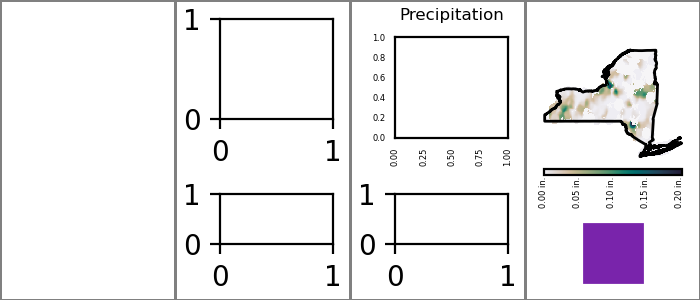
\includegraphics[width=2.5in]{k_different_types.png}
\end{figure}


We care about continuity b/c 
\begin{figure}
  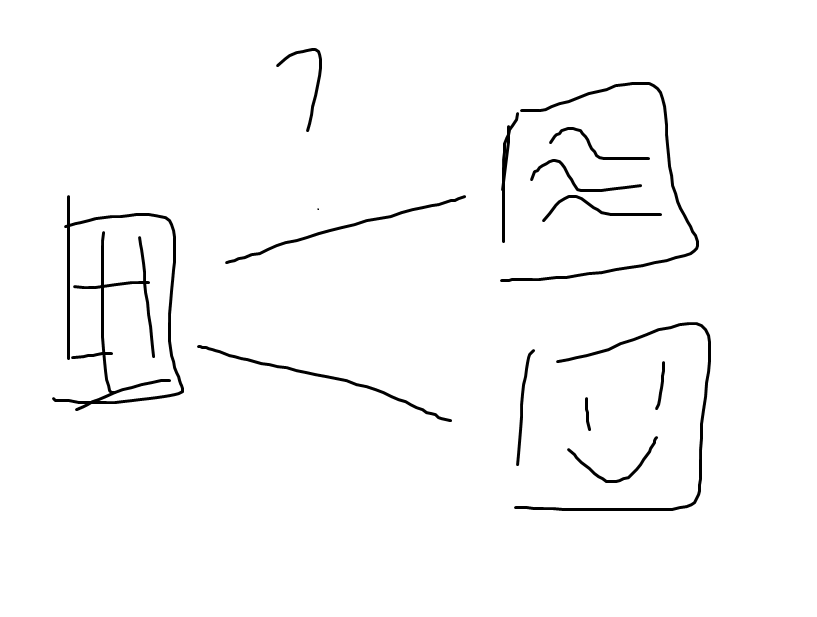
\includegraphics[width=2.5in]{whycontinuity.png}
\end{figure}

We express continuity using fiber bundles, which are ...
\cite{butlerVectorBundleClassesForm1992,butlerVisualizationModelBased1989}
\begin{equation}
  \label{eq:fiber_bundle}
  \begin{tikzcd}
      \dfiber \arrow[r, hook] & \dtotal \arrow[r, "\pi"] & \dbase
  \end{tikzcd}
\end{equation}



\subsection{Equivariance}
What is it?

\begin{figure}[!h]
  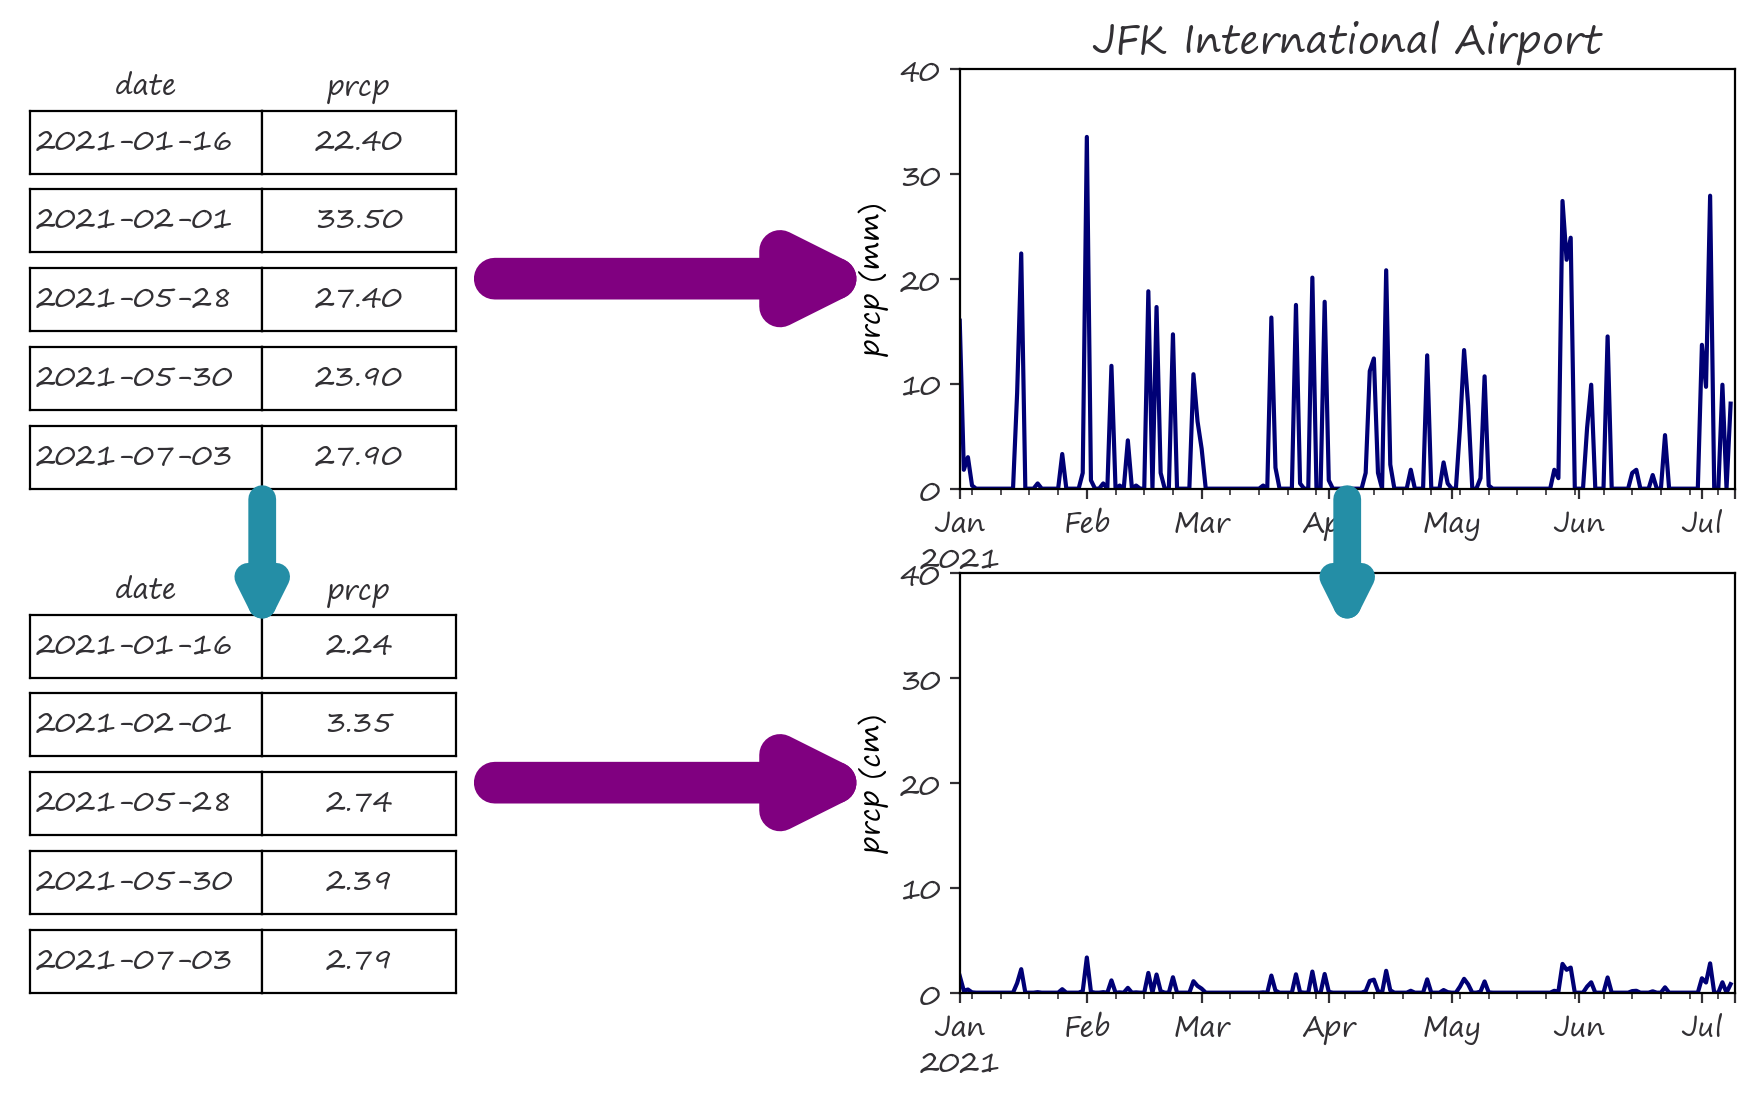
\includegraphics[width=2.5in]{equiv.png}
\end{figure}

\begin{tikzcd}
  data \arrow[r] \arrow[d, "function"] & representation \arrow[r] & visual\;stimulus \arrow[d, "visual\;equivalent\;to\;function"] \\
  data \arrow[r]                       & representation \arrow[r] & visual\; stimulus                                          
\end{tikzcd}

\section{Topological Equivariant Artist Model}
%%- brief intro to artist in most simple form $\vartist \dtotal \rightarrow \gtotal$ 

\section{Union of Artists}
\begin{figure}[!h]
\centering
\subfloat[Artists with shared $\mu_i$ renderered correctly]{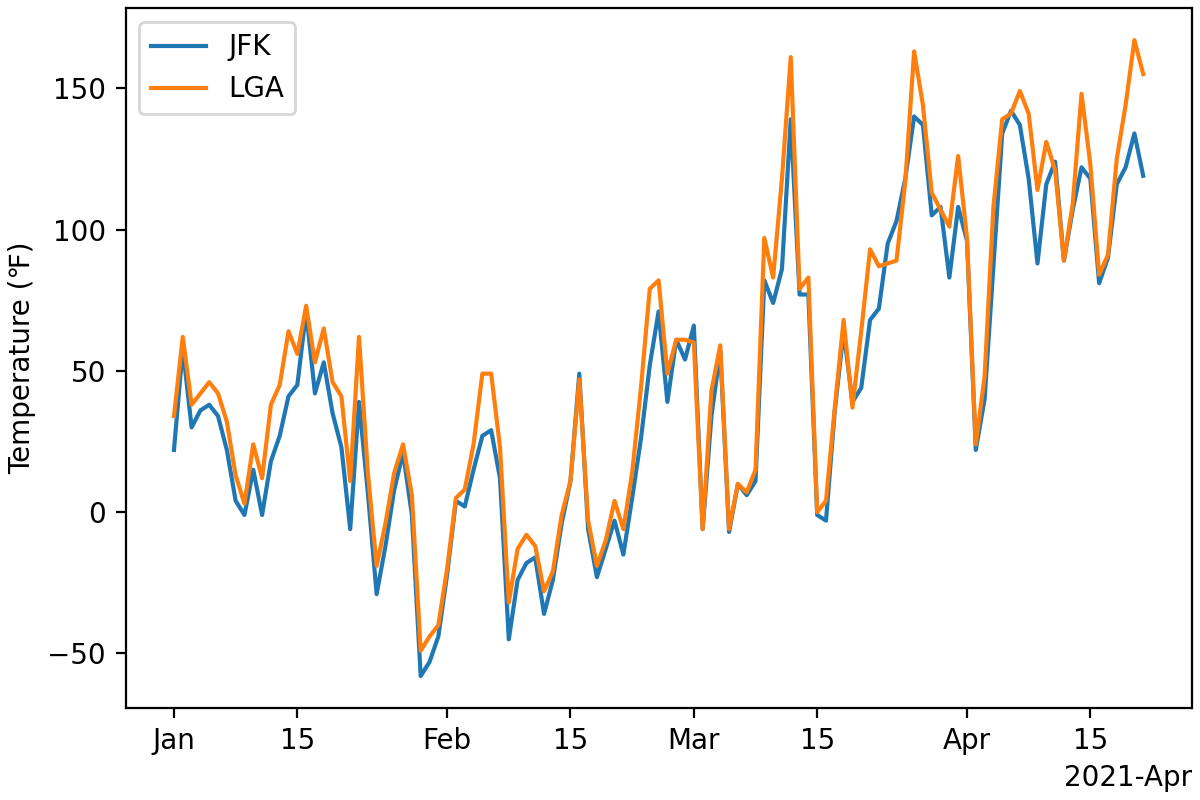
\includegraphics[width=1.2in]{combined_artist.png}%
\label{fig_first_case}}
%\hfil
\subfloat[Artists without shared $\mu_i$]{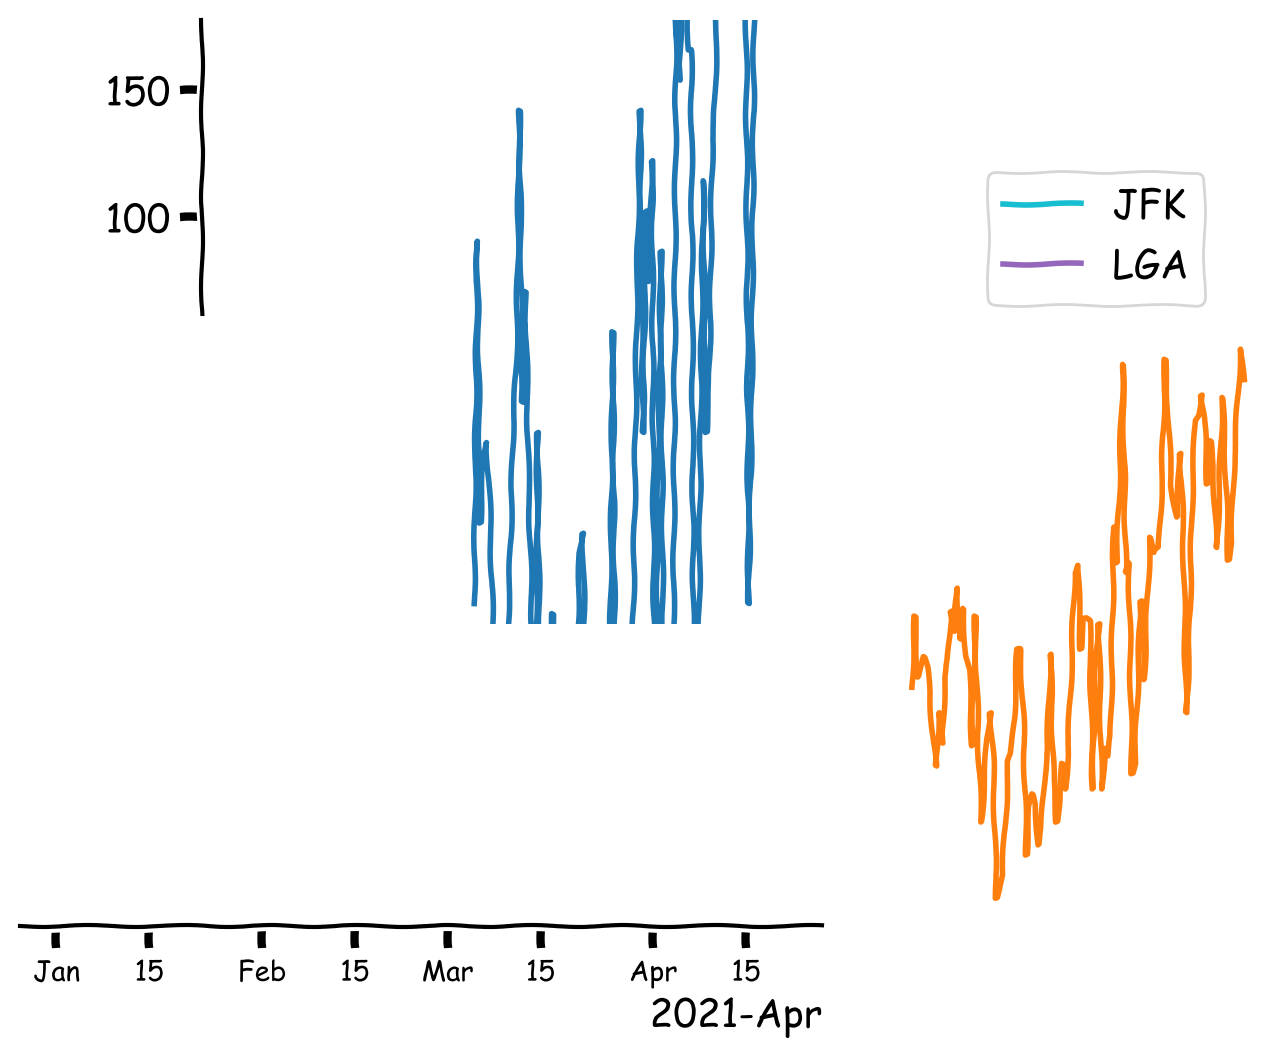
\includegraphics[width=1.2in]{exploding_artist.png}%
\label{fig_second_case}}
\caption{Simulation results for the network.}
\label{fig_sim}
\end{figure}
}


\subsection{Data Bundle \dtotal}
\begin{figure}[!h]
  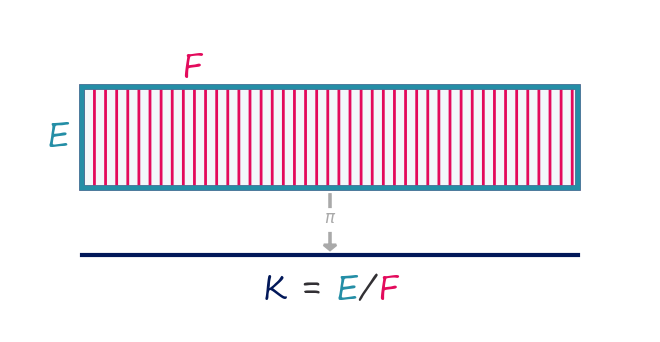
\includegraphics[width=2.5in]{k_qspace.png}
  \caption{this is gonna be replaced w/ more concrete}
\end{figure}

\paragraph{Structured Data: Section \dsection}
\begin{equation}
  \begin{tikzcd}
      \dfiber \arrow[r, hook] & \dtotal \arrow[d, "\pi"'] \\
                        & \dbase \arrow[u, "\dsection"', bend right]
  \end{tikzcd}
\end{equation}

\paragraph{Structure: Continuity and Equivariant Actions}
\begin{equation}
  \begin{tikzcd}
      \dfiber_i \arrow[d, "m_j"'] \arrow[rd, "m_j\;\circ\; m_k"] &         \\
      \dfiber_i \arrow[r, "m_k"']  & \dfiber_i
  \end{tikzcd}
\end{equation}

\subsubsection{Continuity of Data: sheaf \sheaf}
\begin{figure}
  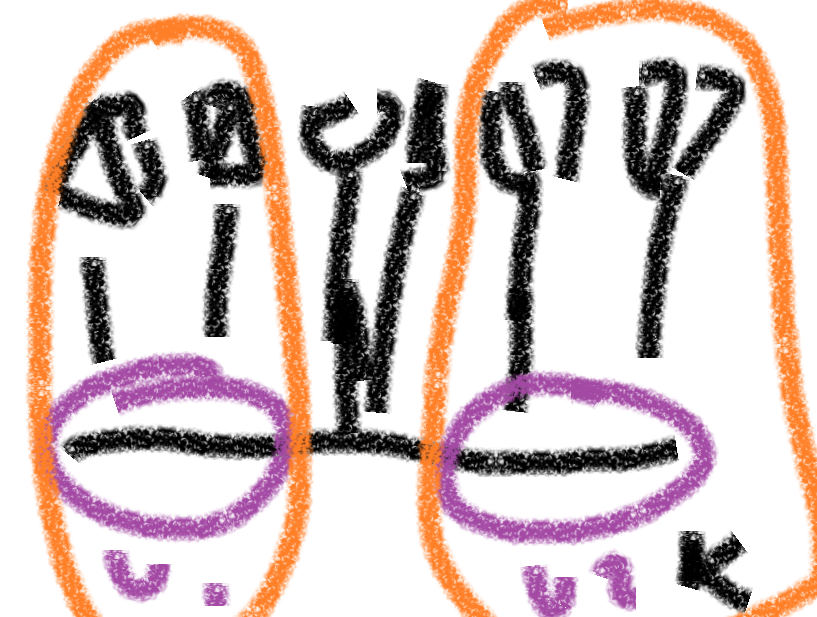
\includegraphics[width=2.5in]{sheaf.png}
  \caption{Maybe create a figure that shows what the sheaf does, like 
  https://www.euclideanspace.com/maths/topology/sheaf/index.htm}
\end{figure}

\subsection{Graphic Bundle \gtotal} %probably doesn't all need to be subsections, just figure + short description
\begin{figure}
  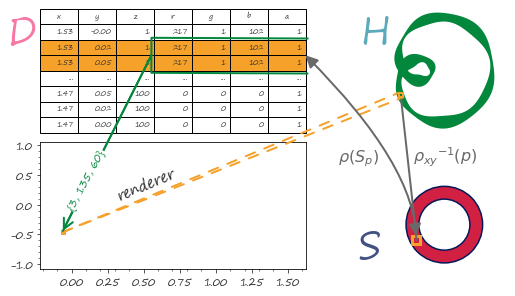
\includegraphics[width=2.5in]{render.png}
\end{figure}
\begin{equation}
  \begin{tikzcd}[ampersand replacement=\&]
      \gfiber \arrow[r, hook] \& \gtotal \arrow[d, "\pi"'] \\
                        \& \gbase \arrow[u, "\gsection"', bend right]
  \end{tikzcd}
\end{equation}
\paragraph{Continuity: Base Space \gbase}
\paragraph{Equivariance: Fiber \gfiber}
\paragraph{Structured Data: Visual \gsection}

\subsection{Artist}
%% flesh out categorical framing of artist, walk through how eq 16 is part of implementing the artists
%% https://github.com/story645/proposal/blob/main/notes/meetings/2021_08_30.md
\begin{equation}
  \vartist: \sheaf(\dtotal) \rightarrow \sheaf(\gtotal)
  \label{eq:math:artist:artist}
\end{equation}


\subsubsection{Graphic to Data: \vindex}
\begin{figure}[!h]
  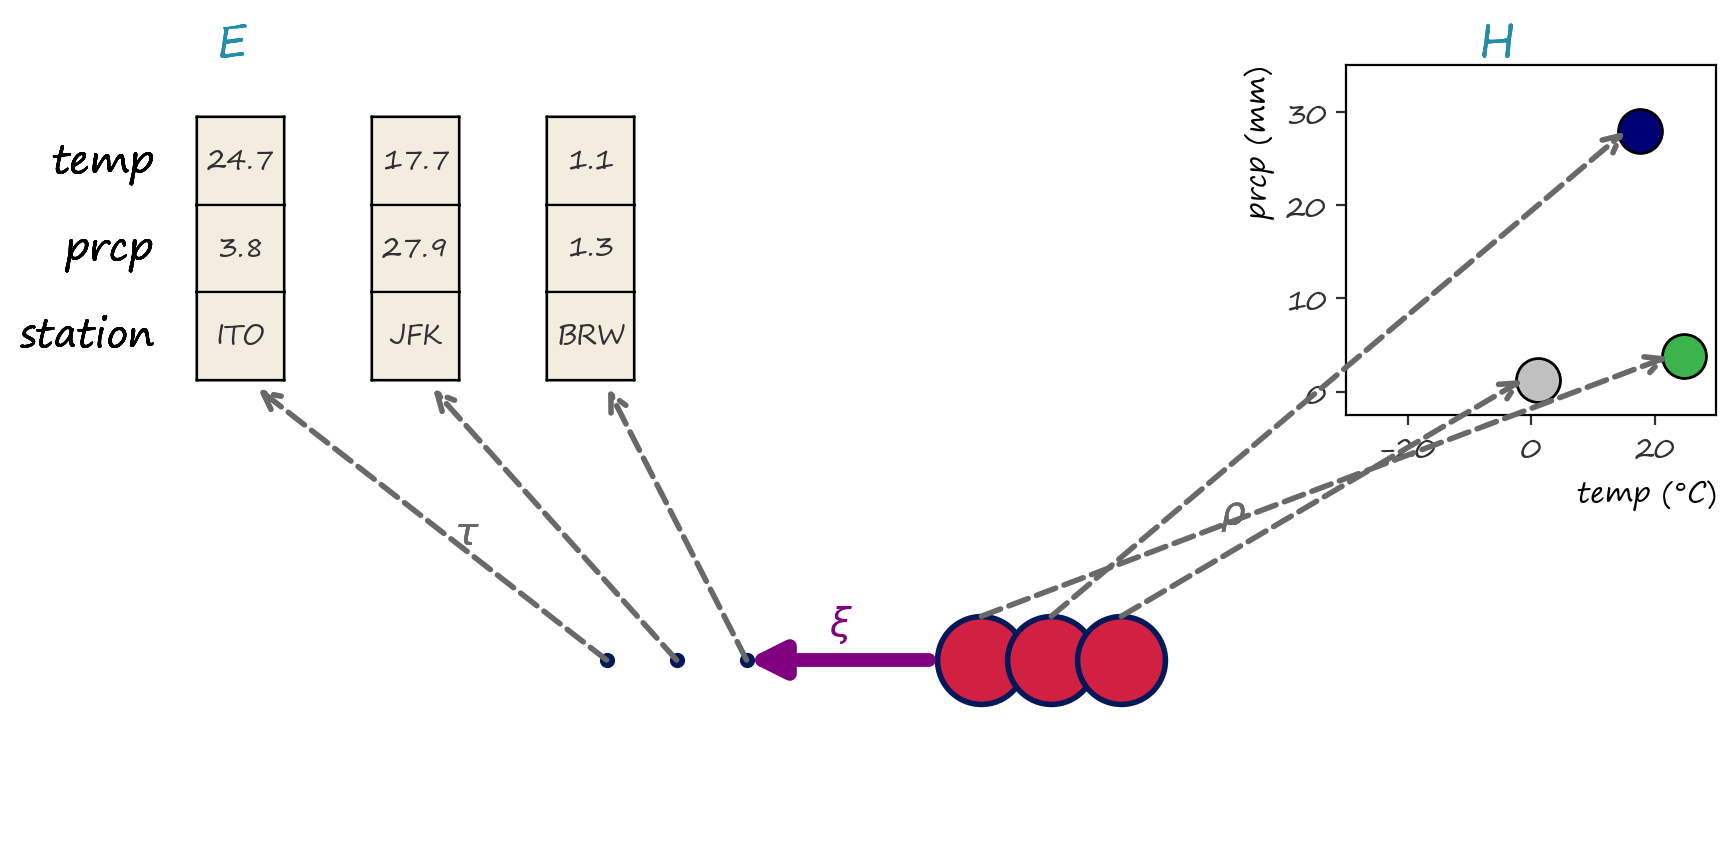
\includegraphics[width=2.5in]{xi.png}
\end{figure}
\begin{equation}
  \begin{tikzcd}
      \dtotal \arrow[d, "\pi"'] & \gtotal \arrow[d, "\pi"'] \\
      \dbase                   & \gbase \arrow[l, "\vindex"']
  \end{tikzcd}
  \label{eq:math:graphic:vindex}
\end{equation}

\begin{equation}
  \label{eq:math:artist:diagram}
  \begin{tikzcd}
      \dtotal \arrow[r, "\vchannel"] \arrow[rd, "\pi"'] & \vtotal \arrow[d, "\pi"] & \vindex^*\vtotal \arrow[r, "\vmark"] \arrow[d, "\vindex^*\pi"'] \arrow[l, "\vindex^*"'] & \gtotal \arrow[ld, "\pi"] \\
                                            & \dbase                  & \gbase \arrow[l, "\vindex"']                                              &                    
      \end{tikzcd}
\end{equation}

\subsubsection{Representation \vtotal}
\begin{equation}
  \begin{tikzcd}[ampersand replacement=\&]
      \vfiber \arrow[r, hook] \& \vtotal \arrow[d, "\pi"'] \\
                        \& \dbase \arrow[u, "\vsection"', bend right]
  \end{tikzcd}
\end{equation}

\subsubsection{Data to Representation: \vchannel} %look at what K&S call these stages
\begin{figure}[!h]
  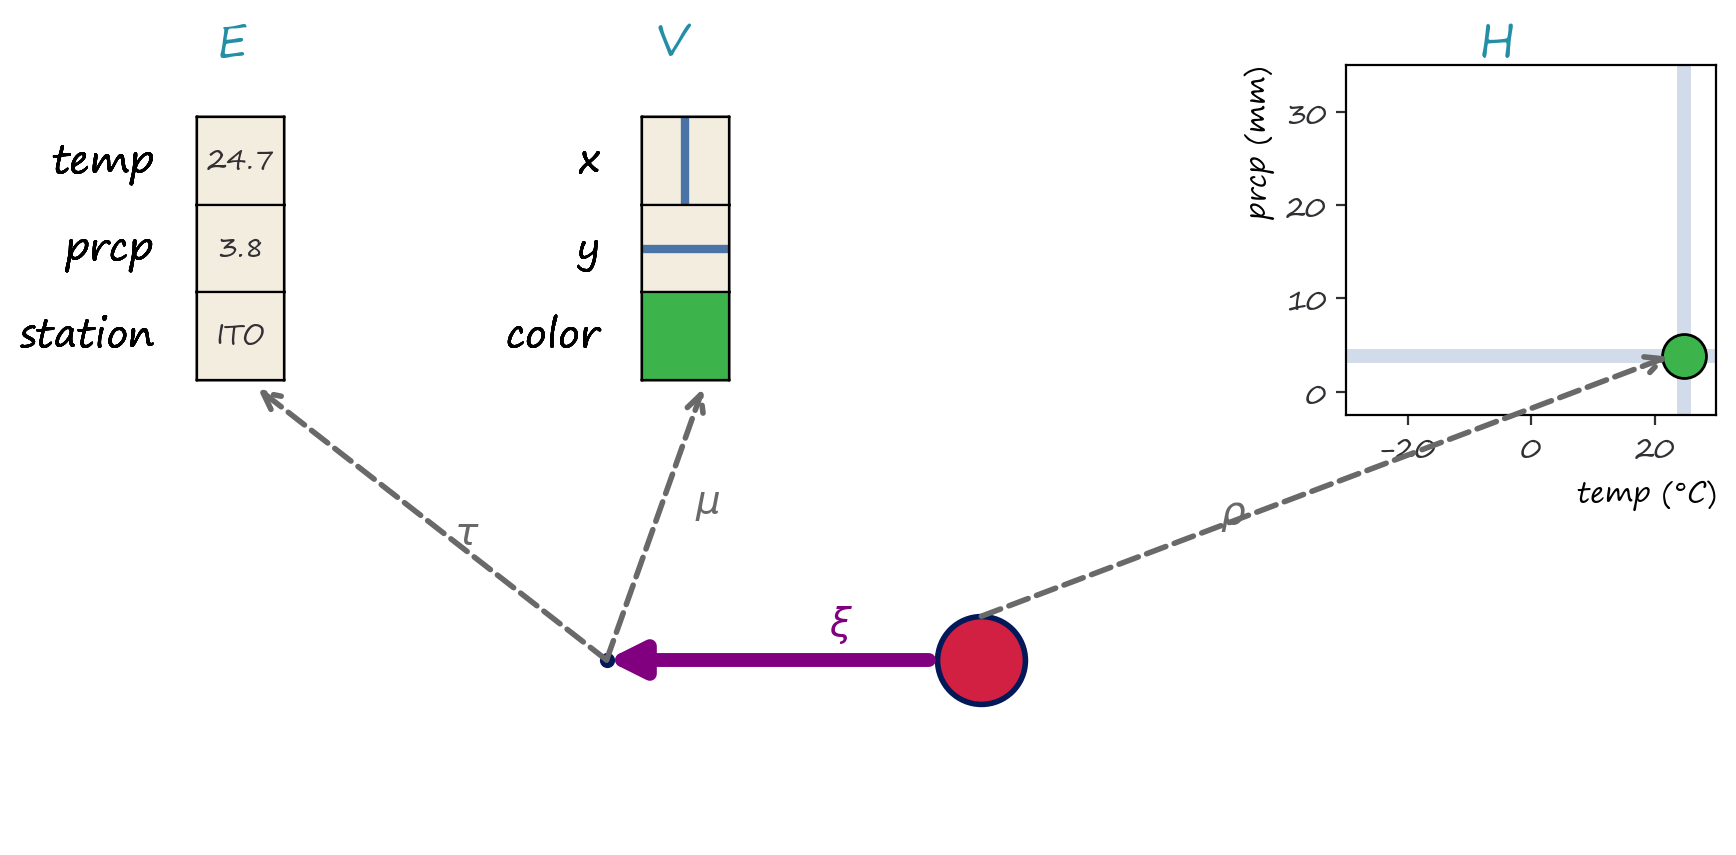
\includegraphics[width=2.5in]{nu.png}
\end{figure}
\begin{equation}
  \label{eq:math:artist:nu}
  \{\vchannel_{0}, \ldots, \vchannel_{n}\}: \{\dsection_{0}, \ldots, \dsection_{n}\} \mapsto \{\vsection_{0}, \ldots, \vsection_{n}\}
\end{equation}

We enforce the equivariance constraint
\begin{equation}
  \label{eq:math:artist:nu_commute}
\begin{tikzcd}
  \dtotal_i \arrow[r] \arrow[r, "\vchannel_i"] \arrow[d, "m_{\delement}"'] & \vtotal_i \arrow[d, "m_{\velement}"] \\
  \dtotal_i \arrow[r, "\vchannel_i"]                           & \vtotal_i               
\end{tikzcd}
\end{equation}

\subsubsection{Representation to Visual: \vmark} % look at what K&S call these stages

\begin{figure}[!h]
  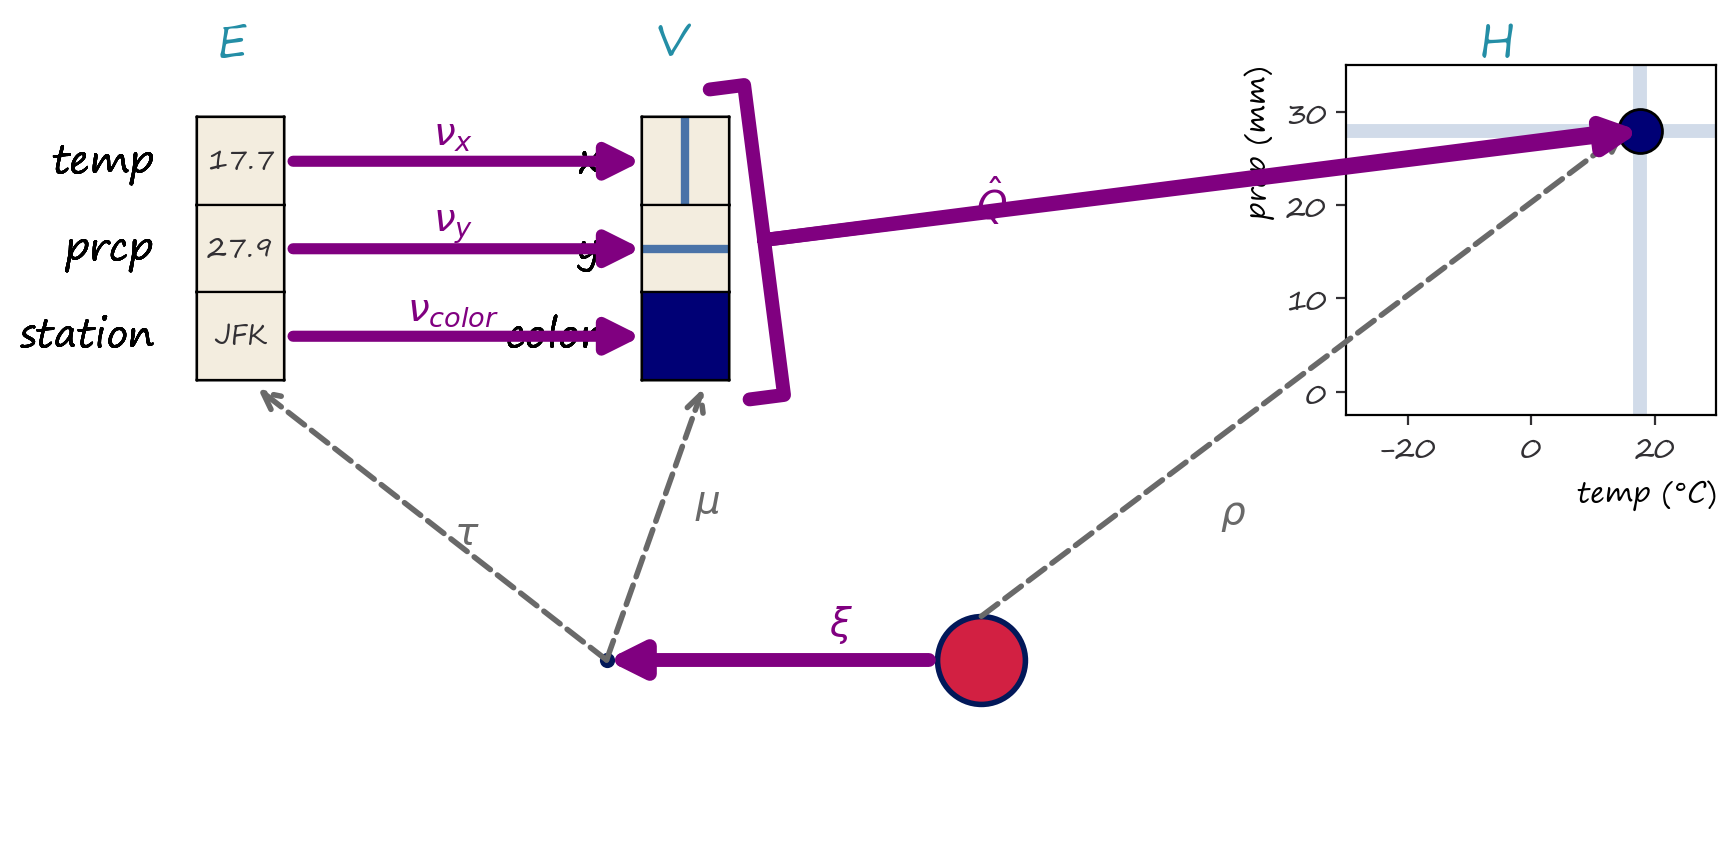
\includegraphics[width=2.5in]{q.png}
\end{figure}

\begin{figure}[!h]
  
\includegraphics[width=2.5in]{diff_type_q.png}
  \caption{rework this as a commutative box w/ the r in E row associated w/ this qhat(k)}
\end{figure}
 
\subsubsection{Data $\leftrightarrow$ Visual}
Putting all the pieces together, we have a system for 
\begin{equation}
  \label{eq:math:artist:diagram}
  \begin{tikzcd}
      \dtotal \arrow[r, "\vchannel"] \arrow[rd, "\pi"'] & \vtotal \arrow[d, "\pi"] & \vindex^*\vtotal \arrow[r, "\vmark"] \arrow[d, "\vindex^*\pi"'] \arrow[l, "\vindex^*"'] & \gtotal \arrow[ld, "\pi"] \\
                                            & \dbase                  & \gbase \arrow[l, "\vindex"']                                              &                    
      \end{tikzcd}
\end{equation}

\section{Case Study}
\begin{figure}[t!]
  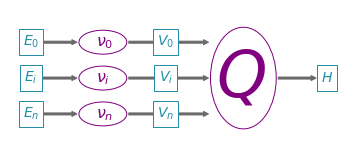
\includegraphics[width=2.5in]{path_of_q.png}
    \caption{add in xi!}
  \label{fig:api}
\end{figure}
We implement the \texbf{arrows} in \autoref{fig:api} 



\section{Discussion}
\subsection{Limitations}
\subsection{future work}

\section{Conclusion}
The conclusion goes here.


\appendices
\section{Rendering: \gsection}
\section{Manufacturing $\vmarkd \leftarrow \vmark$}
\begin{equation}
  \begin{tikzcd}
      \textcolor{gray!50}{\dtotal} \arrow[r, "\vchannel", color=gray!50] \arrow[rd, "\pi"', color=gray!50] & \vtotal \arrow[d, "\pi"']                  & \vindex^*\vtotal \arrow[r, "\vmark", color=gray!50] \arrow[d, "\vindex^*\pi"'] \arrow[l,  "\vindex^*"'] & \textcolor{gray!50}{\gtotal} \arrow[ld, "\pi", color=gray!50] \\ & \dbase \arrow[u, "\vsection"', bend right] & \gbase \arrow[l, "\vindex"'] \arrow[u, "\vindex^*\vsection"', bend right]               &                          
      \end{tikzcd}
      \label{eq:math:artist:qhat}
\end{equation}



% use section* for acknowledgment
\ifCLASSOPTIONcompsoc
  % The Computer Society usually uses the plural form
  \section*{Acknowledgments}
\else
  % regular IEEE prefers the singular form
  \section*{Acknowledgment}
\fi


The authors would like to thank...


% Can use something like this to put references on a page
% by themselves when using endfloat and the captionsoff option.
\ifCLASSOPTIONcaptionsoff
  \newpage
\fi

% trigger a \newpage just before the given reference
% number - used to balance the columns on the last page
% adjust value as needed - may need to be readjusted if
% the document is modified later
%\IEEEtriggeratref{8}
% The "triggered" command can be changed if desired:
%\IEEEtriggercmd{\enlargethispage{-5in}}

% references section

% can use a bibliography generated by BibTeX as a .bbl file
% BibTeX documentation can be easily obtained at:
% http://mirror.ctan.org/biblio/bibtex/contrib/doc/
% The IEEEtran BibTeX style support page is at:
% http://www.michaelshell.org/tex/ieeetran/bibtex/
\bibliographystyle{IEEEtran}
% argument is your BibTeX string definitions and bibliography database(s)
\bibliography{bibliography}


% biography section 
% If you have an EPS/PDF photo (graphicx package needed) extra braces are
% needed around the contents of the optional argument to biography to prevent
% the LaTeX parser from getting confused when it sees the complicated
% \includegraphics command within an optional argument. (You could create
% your own custom macro containing the \includegraphics command to make things
% simpler here.)
%\begin{IEEEbiography}[{\includegraphics[width=1in,height=1.25in,clip,keepaspectratio]{mshell}}]{Michael Shell}
% or if you just want to reserve a space for a photo:

%\begin{IEEEbiography}{Michael Shell}
%\end{IEEEbiography}

% if you will not have a photo at all:
\begin{IEEEbiographynophoto}{Hannah Aizenman}
Biography text here.
\end{IEEEbiographynophoto}

\begin{IEEEbiographynophoto}{Thomas Caswell}
  Biography text here.
\end{IEEEbiographynophoto}
% insert where needed to balance the two columns on the last page with
% biographies
%\newpage

\begin{IEEEbiographynophoto}{Michael Grossberg}
Biography text here.
\end{IEEEbiographynophoto}

% You can push biographies down or up by placing
% a \vfill before or after them. The appropriate
% use of \vfill depends on what kind of text is
% on the last page and whether or not the columns
% are being equalized.

%\vfill

% Can be used to pull up biographies so that the bottom of the last one
% is flush with the other column.
%\enlargethispage{-5in}

% that's all folks
\end{document}


